% 张宇八套卷重新提取勘误（由 build/zy8_errata.py 生成，请勿手改）。
%
% 每份 PDF 只放一个科目；条目按「年份-套次 / 题号：原内容 → 正确内容」给，
% 红色 = 题库原录入，绿色 = 更正后内容。
%
% 依据：对源页 PNG 的原生多模态观察（逐条裁片放大核对），
% 未使用 OCR，未使用 PDF 文本层。
\documentclass[11pt,a4paper]{ctexart}

\usepackage[margin=2.2cm,top=2.6cm]{geometry}
\usepackage{amsmath,amssymb,bm}
\usepackage{tikz}
\usepackage{xcolor}
\usepackage{fancyhdr}
\usepackage{hyperref}

\definecolor{errata-red}{RGB}{198,40,40}
\definecolor{errata-green}{RGB}{20,120,60}

\newcommand{\rc}[1]{\textcolor{errata-red}{#1}}
\newcommand{\gc}[1]{\textcolor{errata-green}{#1}}
\newcommand{\Paper}[1]{\par\vspace{9pt}{\bfseries #1}\par\vspace{3pt}}
\newcommand{\pair}[1]{\par\hangindent=2.2em\hangafter=1 #1\par\vspace{1pt}}

\newcommand{\ErrataSubject}{数学一}

% 题库正文里使用的两个项目宏。勘误文档不排版整卷，只把它们的**印刷形态**画出来，
% 这样勘误条目与原卷面部一致（选择题的括号、填空题的横线）。
\newcommand{\ExamSelection}{（\quad）}
\newcommand{\ExamBlank}{\underline{\hspace{3em}}}

\pagestyle{fancy}
\fancyhf{}
\renewcommand{\headrulewidth}{0pt}
\fancyfoot[C]{\small\thepage}

\setlength{\parindent}{0pt}
\linespread{1.12}
\hypersetup{colorlinks=true,linkcolor=errata-green,urlcolor=errata-green}

\begin{document}

\begin{center}
  {\LARGE\bfseries 张宇八套卷题库勘误清单（\ErrataSubject）}
\end{center}
\vspace{2pt}
\begin{center}
  \small 依据源页逐题回图核对，共 147 处经复核，其中 17 处为题库识别错误并已更正。
\end{center}
\vspace{6pt}
\hrule
\vspace{8pt}

\Paper{2023 张宇八套卷（数学一）第 4 套}
\pair{10：\rc{（整段重录）} $\longrightarrow$ \gc{设总体 $X$ 在 $(a,b)$ 上服从均匀分布，其中 $a,b$ 为未知参数，若对于 $X$ 的一组样本观测值 $x_1,x_2,\cdots,x_{10}$，$a,b$ 的矩估计值分别为 $\hat{a}=2.6,\hat{b}=6.2$，则该样本的样本方差为\ExamSelection}}
\pair{13：\rc{（整段重录）} $\longrightarrow$ \gc{曲线 $y=e^{-\frac{x}{2}}\sqrt{\sin x}$ 在 $[0,2\pi]$ 部分与 $x$ 轴围成的图形绕 $x$ 轴旋转一周所成的旋转体的体积为 $\ExamBlank$。}}
\Paper{2023 张宇八套卷（数学一）第 6 套}
\pair{21：\rc{（整段重录）} $\longrightarrow$ \gc{求 $A^*-6E$ 的秩。}}
\Paper{2023 张宇八套卷（数学一）第 8 套}
\pair{8：\rc{（整段重录）} $\longrightarrow$ \gc{$U^{\alpha+1}$}}
\Paper{2024 张宇八套卷（数学一）第 5 套}
\pair{1：\rc{（整段重录）} $\longrightarrow$ \gc{函数 $f(x)=\dfrac{x|x-1|}{\sin\pi x}$ 的可去间断点的个数为\ExamSelection}}
\Paper{2024 张宇八套卷（数学一）第 7 套}
\pair{2：\rc{（整段重录）} $\longrightarrow$ \gc{$f''_{yx}(0,0)=1$}}
\pair{19：\rc{（整段重录）} $\longrightarrow$ \gc{存在 $\xi\in(0,1)$，使得 $f'(\xi)<2$；}}
\Paper{2025 张宇八套卷（数学一）第 5 套}
\pair{8：\rc{（整段重录）} $\longrightarrow$ \gc{$P(\overline{A}\,\overline{B})>P(\overline{A})P(\overline{B})$。}}
\pair{8：\rc{（整段重录）} $\longrightarrow$ \gc{设随机事件 $A,B$ 满足 $0<P(A)<1,0<P(B)<1$，则 $P(AB)>P(A)P(B)$ 的充要条件是\ExamSelection}}
\Paper{2025 张宇八套卷（数学一）第 6 套}
\pair{7：\rc{（整段重录）} $\longrightarrow$ \gc{$r(\boldsymbol{A}\ \ \boldsymbol{AB})=r(\boldsymbol{A})$。}}
\pair{7：\rc{（整段重录）} $\longrightarrow$ \gc{$r\left(\boldsymbol{AB}^\mathrm{T}\ \ \boldsymbol{AB}^\mathrm{T}\boldsymbol{B}\right)=r(\boldsymbol{AB}^\mathrm{T})$。}}
\pair{7：\rc{（整段重录）} $\longrightarrow$ \gc{$r\begin{pmatrix}\boldsymbol{A}^\mathrm{T}\boldsymbol{A}\\\boldsymbol{B}^\mathrm{T}\boldsymbol{A}\end{pmatrix}=r(\boldsymbol{A})$。}}
\pair{8：\rc{（整段重录）} $\longrightarrow$ \gc{$AC=\varnothing$。}}
\Paper{2026 张宇八套卷（数学一）第 3 套}
\pair{5：\rc{（整段重录）} $\longrightarrow$ \gc{$AP_2^{\mathrm T}P_1^9=B$。}}
\pair{7：\rc{（整段重录）} $\longrightarrow$ \gc{设 $A$ 为 $n$ 阶方阵，有下列结论：
①若 $A$ 的全部顺序主子式为正，则 $A$ 正定；
②若 $A$ 相似于对角矩阵 $\Lambda$，则 $A$ 与 $\Lambda$ 合同；
③若 $A$ 与正定矩阵合同，则 $A$ 为正定矩阵。
则正确结论的个数为\ExamSelection}}
\Paper{2026 张宇八套卷（数学一）第 4 套}
\pair{4：\rc{（整段重录）} $\longrightarrow$ \gc{若级数 $\sum_{n=1}^{\infty}|u_nv_n|$ 发散，则\ExamSelection}}
\pair{7：\rc{（整段重录）} $\longrightarrow$ \gc{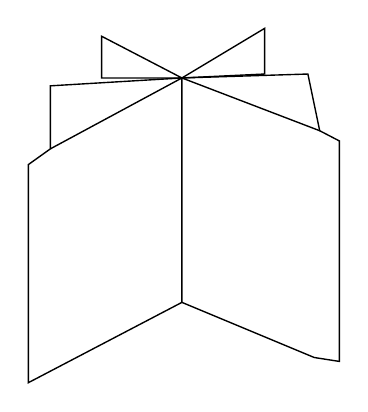
\begin{tikzpicture}[scale=1.0,line width=0.5pt]
% P 为三张平面的公共点，Q 为公共棱的下端（PQ 即公共交线）
\coordinate (P) at (2.15,4.35);
\coordinate (Q) at (2.15,1.50);
% 左侧平面（外侧棱上有一处折角）
\draw (0.48,4.25) -- (P) -- (Q) -- (0.20,0.48) -- (0.20,3.25) -- (0.48,3.45) -- cycle;
% 右侧平面（外侧棱上有一处折角）
\draw (P) -- (3.75,4.40) -- (3.90,3.68) -- (4.15,3.55) -- (4.15,0.75) -- (3.83,0.80) -- (Q);
% 第三个平面在左右两平面上的交线
\draw (P) -- (0.48,3.45);
\draw (P) -- (3.90,3.68);
% P 上方左右两个三角形面片
\draw (1.13,4.88) -- (1.13,4.35) -- (P) -- cycle;
\draw (3.20,4.98) -- (3.20,4.40) -- (P) -- cycle;
\end{tikzpicture}}}

\end{document}
